\subsection{Experiment 3: Overlooking Experimental Block Effects Can Lead to Biased Model Performance Estimates}

\begin{figure}[H]
    \centering
    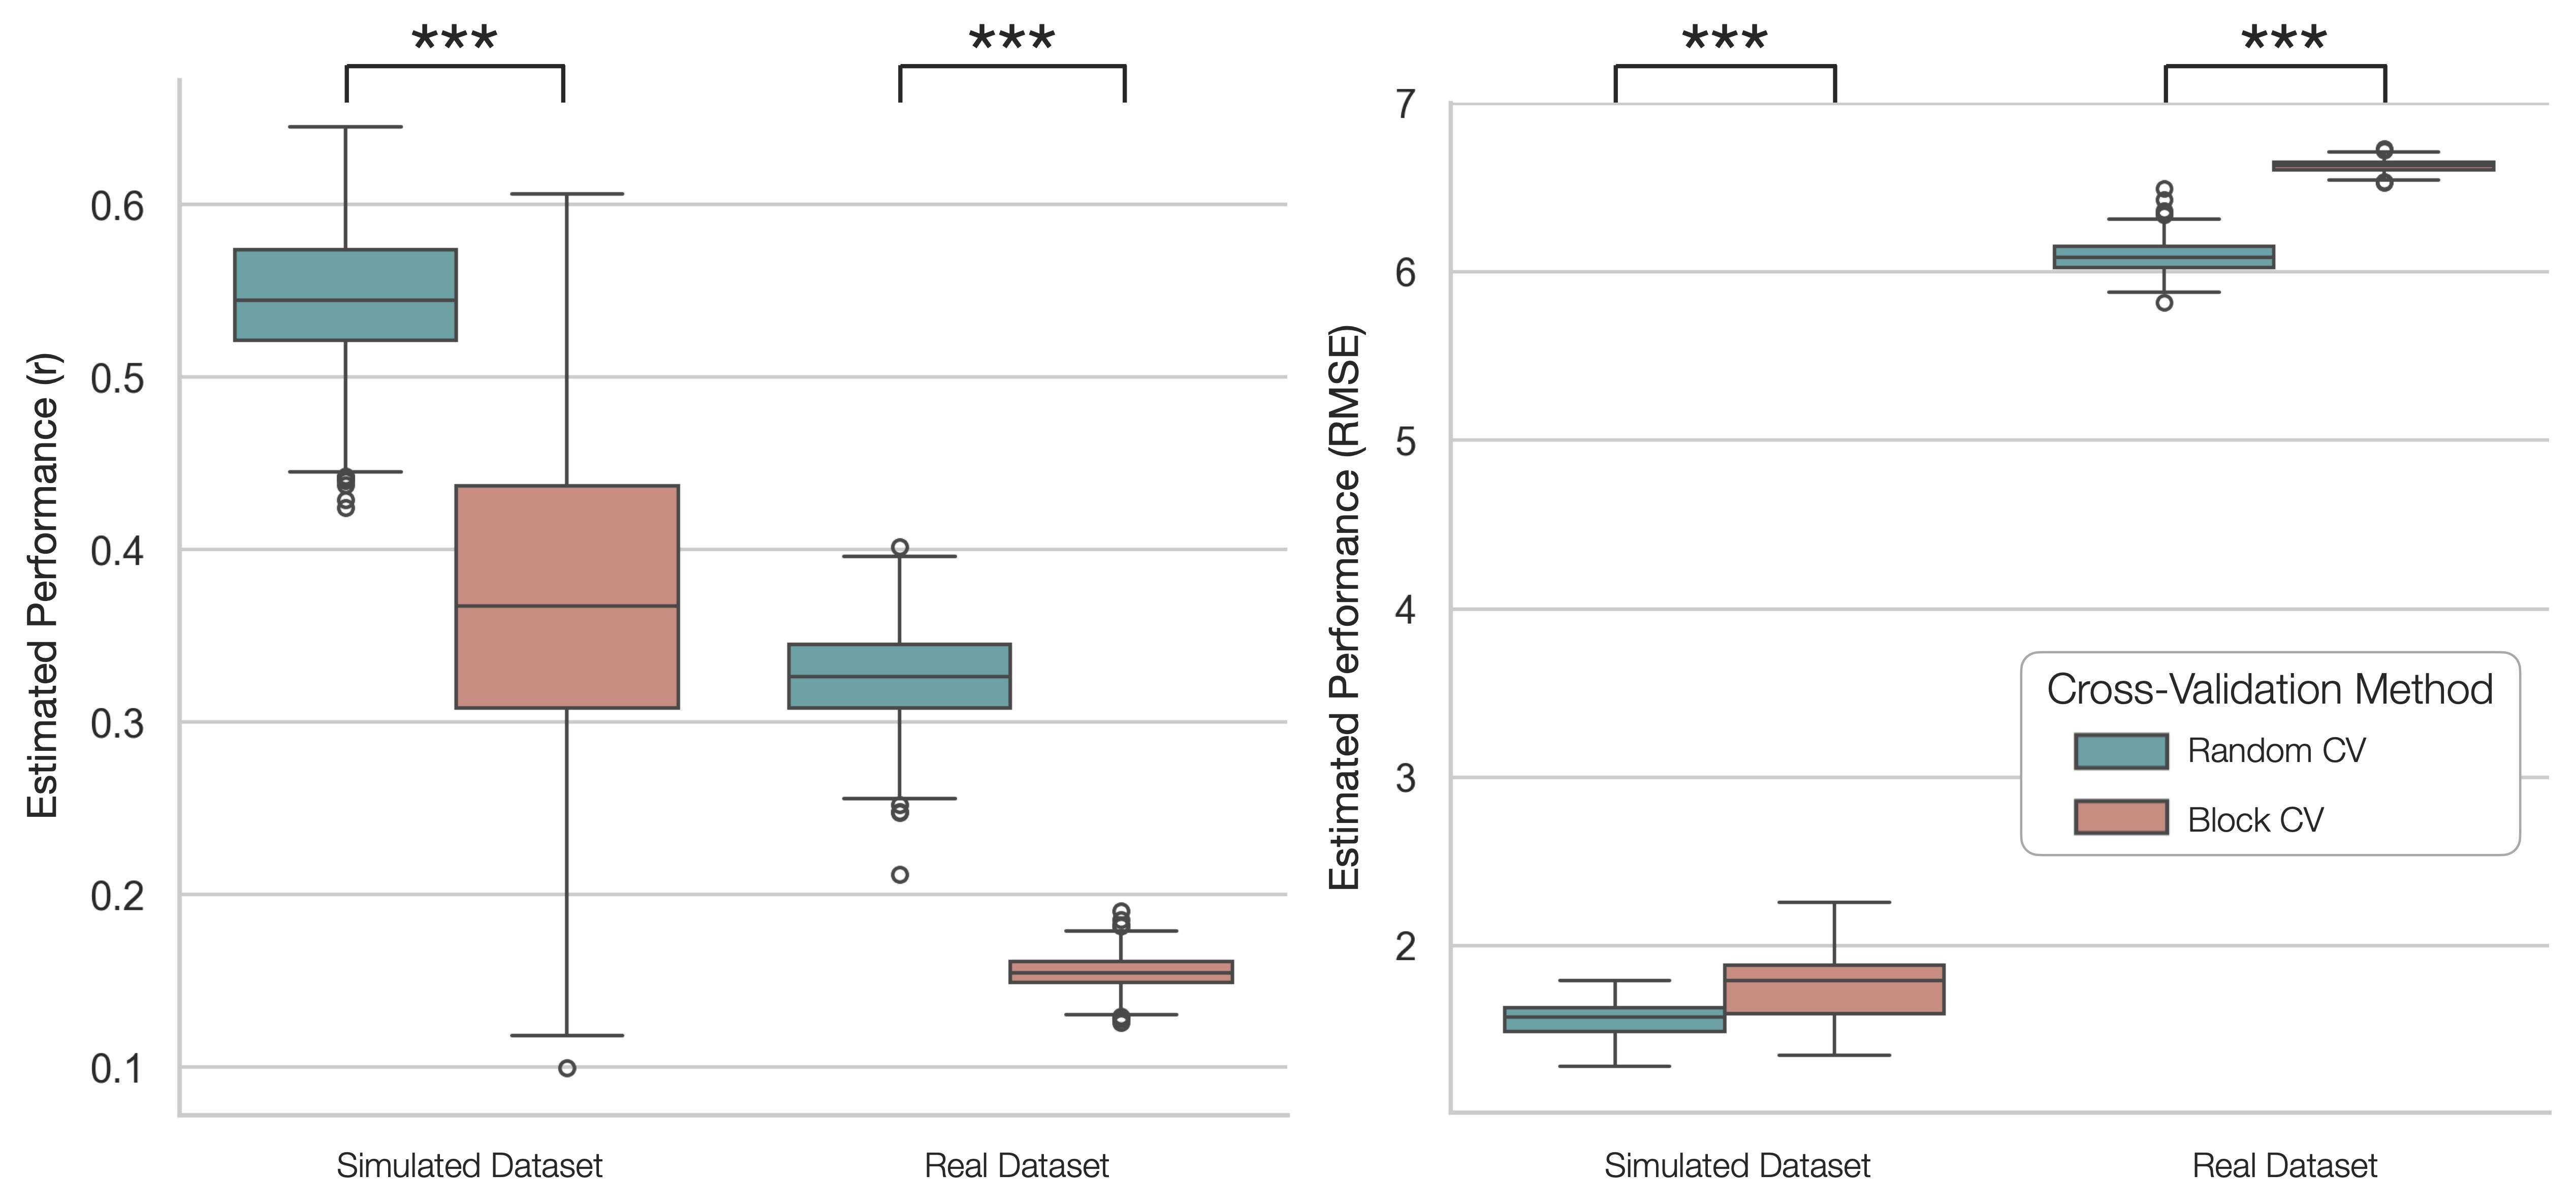
\includegraphics[width=1\textwidth]{fig_8.jpg}
    \caption{Over-estimation of model performance by Random CV compared to Block CV demonstrated in metrics of Pearson's correlation $r$ (left) and root mean squared error, RMSE (right). The significant difference is noted as ***, p-value < 0.00001.}
    \label{fig:s3_results}
\end{figure}

Performance inflation is evident in both the simulated and real spectral datasets, which inherently exhibit seasonal variation as block effects (Figure~\ref{fig:s3_results} and Table~\ref{tab:anova_all}). Ignoring this seasonal variation leads to a notable overestimation of model performance, as reflected by a 17.5\% bias in r for the simulated dataset and 17.1\% for the real dataset. A similar pattern emerges for RMSE, with a 15.5\% bias in the simulated dataset and an 11.1\% bias in the real dataset. The ANOVA results further support these findings, since all four tests show significant differences (p-value < 0.001) between the two methods on the estimated model performance.

St-Pierre (2001) made a similar observation when comparing datasets collected from different studies conducted under distinct time periods or environmental conditions \citep{st-pierre_invited_2001}. The distinctness often manifests in differences in variance or value scales, complicating comparisons in the literature. St-Pierre defined this phenomenon as the “study effect,” recommending that it be calibrated as a random variable instead of a fixed variable in a linear mixed model. It is because these study effects are unobserved until the data is collected, fitting these effects as random variables allows for the calibration of a broader set of study effects, including those that are unobserved. The author advocated for calibrating the study variation before making any inferences from the dataset, which parallels the need to calibrate the seasonal variation in prediction modeling to alleviate the overestimation bias observed in random CV.

Similar discussion are found in maize breeding. Predicting hybrid yield performance for future years or seasons has been a challenge. De Oliveira et al. (2020) estimated hybrid performance across multiple years and compared two CV systems \citep{de_oliveira_genomic_2020}. The first system used random splits of the available hybrids into validation folds, while the second employed year-based splits, which is an approach akin to block CV as advocated in this study. The results showed substantial performance differences of up to 0.4 in $r$ across years, underscoring the impact of properly accounting for temporal effects. Since seasons are inherently random effects that cannot be fully observed in historical datasets (as no two seasons are identical in their environmental responses to yield), a common strategy to address this issue is to quantify year-to-year variation using quantitative variables rather than directly modeling the seasonal effect. In crop modeling, such variables are referred to as environmental covariates, which decompose environmental variability into measurable components like temperature, humidity, and soil moisture. For instance, Cruz et al. (2023) incorporated 183 environmental covariates, including cumulative thermal time, soil water evaporation, leaf area index, and daily infiltration, into their prediction models \citep{lopez-cruz_leveraging_2023}. By estimating the effects of these covariates, researchers can address the missing information from unseen seasonal variations and mitigate the performance drop when transitioning from random CV to block CV.

Another perspective to explain the discrepancy between the evaluated performance and the actual performance is the inherent domain shift that can occur between training and deployment conditions, especially in agriculture, where climate, soil types, and management practices may differ significantly across regions. This challenge is further complicated by imperfect data sampling and model variability. Any dataset is merely a partial reflection of real-world conditions, and different models trained on the same dataset can learn markedly different decision boundaries due to noise, bias, or sparsity \citep{renard_understanding_2024}. Even when those models achieve similar predictive performance according to standard metrics, they may still exhibit a multiplicity of equally performing models, meaning they classify individual instances differently in ambiguous parts of the feature space. Consequently, relying exclusively on conventional performance metrics (e.g., RMSE, MAE) can sometimes be misleading for real-world applications.

For instance, in the energy sector, one study predicting cooling loads for an ice-based thermal energy storage system compared 180 models using traditional measures, finding that the top performer under these metrics was not the most effective when actually deployed to control the system. Such findings emphasize the importance of going beyond standard accuracy measures \citep{wang_investigating_2024}. 

To address such domain shift in remote-sensing-based crop yield prediction, for example, recent work has proposed a multisource maximum predictor discrepancy (MMPD) neural network, which aligns source and target domains while mitigating negative interference among multiple training sources \citep{ma_multisource_2023}. By maximizing the discrepancy between source-specific yield predictors while considering the unlabeled target domain, this approach effectively reduces domain shift and has been shown to outperform various state-of-the-art deep learning and unsupervised domain adaptation methods.

These observations emphasize the importance of closely examining identifiable sources of variation in experiments and aligning evaluation strategies with the model’s intended real-world application. Variations, such as seasonal block effects, can simultaneously influence both predictive features and response variables. If a model is intended for deployment in a new block, such as a future season for which no prior information is available, using block CV is critical to ensure the evaluation results in generalizability. Conversely, for models designed for a closed environment where all possible blocks are represented, random CV may offer a more efficient evaluation strategy.
